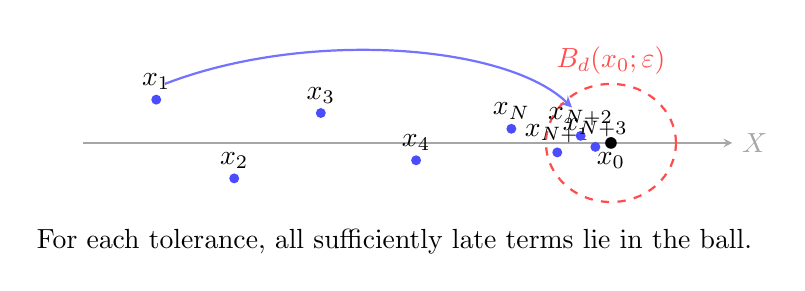
\begin{tikzpicture}[x=1.1cm,y=1cm,>=stealth]
  \draw[->,gray!70] (-0.4,0) -- (7.1,0) node[right] {\(X\)};
  \fill[black] (5.7,0) circle (2.1pt);
  \node[below] at (5.7,0) {\(x_0\)};

  \draw[red!70,thick,dashed] (5.7,0) circle (0.75);
  \node[red!70] at (5.7,1.05) {\(B_d(x_0;\varepsilon)\)};

  \foreach \x/\y/\lab in {
    0.45/0.55/x_1,
    1.35/-0.45/x_2,
    2.35/0.38/x_3,
    3.45/-0.22/x_4,
    4.55/0.18/x_N,
    5.08/-0.12/x_{N+1},
    5.35/0.09/x_{N+2},
    5.52/-0.05/x_{N+3}
  }
  {
    \fill[blue!70] (\x,\y) circle (1.8pt);
    \node[above] at (\x,\y) {\(\lab\)};
  }

  \draw[->,blue!55,thick] (0.55,0.75) .. controls (2.2,1.45) and (4.5,1.25) .. (5.25,0.45);
  \node[align=center] at (3.2,-1.25)
    {For each tolerance, all sufficiently late terms lie in the ball.};
\end{tikzpicture}
